\documentclass[final]{article}
\usepackage{main}
\title{Distributed Algorithms for Connectivity and MST in Large Graphs with Efficient Local Computation}
\author{Eric Ajieren, Khalid Hourani, William K. Moses Jr., Gopal Pandurangan}
\date{}

\begin{document}
\maketitle
\begin{abstract}
    We study distributed algorithms for large-scale graphs, focusing on the
    fundamental problems of connectivity and minimum spanning tree (MST). We
    consider the \(k\)-machine model, a well-studied model for distributed
    computing for large-scale graph computations, where \(k \geq 2\) machines
    jointly perform computations on graphs with \(n\) nodes (typically, \(n \gg
    k\)). The input graph is assumed to be initially randomly partitioned among
    the \(k\) machines, a common implementation in many real-world systems.
    Communication is point-to-point, and the goal is to minimize the number of
    \emph{communication rounds} (denoted \(T_c\)) of the computation.

    While communication is a significant factor that affects the time needed for
    large-scale computations, the \emph{computation cost} incurred by the
    individual machines also contributes to the overall time complexity of the
    distributed algorithm. We posit a complexity measure called the \emph{local
    computation cost} (denoted \(T_{\ell}\)) that measures the worst-case local
    computation cost among the machines.  A lower bound for \(T_{\ell}\)
	in our model is \(\bigOm{\sfrac{(m+n)}{k} + \Delta + k}\), while a
    lower bound on \(T_c\) is \(\bigOm{\sfrac{n}{k^2}}\) [Klauck et al., SODA 2015],
    where $m$ is the number of edges and $\Delta$ is the maximum degree. Prior
    algorithms for connectivity and MST in the $k$-machine model [Klauck et al.,
    SODA 2015, Pandurangan et al., SPAA 2016] do not take into account local
    computation; a straightforward local implementation of these algorithms is
    not optimal with respect to local computation.

    In this paper, we study several distributed algorithms for connectivity and
    MST and analyze their performance with respect to \emph{both} the computation and
    communication cost. In particular, we analyze a well-studied flooding
    algorithm for connectivity and connected components that takes
    \(\softO{n/k + D}\) rounds and \(\softO{m / k + \Delta + k}\)
    local computation time.\footnote{\(\tilde{\mathcal{O}}\) notation hides
    \(\operatorname{polylog}(n)\) multiplicative and additive factors.} We then
    present a deterministic filtering algorithm that has an improved
    round complexity of \(\softO{\sfrac{n}{k}}\) but local computation
    complexity of \(\softO{\sfrac{m}{k} + n}\). Next, we present two
    \emph{deterministic} algorithms which are increasingly sophisticated
    implementations of the classical Bor\r{u}vka's algorithm, the last of which
    has round complexity \(\softO{\sfrac{n}{k}}\) and local computation
    complexity \(\softO{\sfrac{(m + n)}{k} + \Delta + k}\). We finally
    present a \emph{randomized} algorithm to find connected components with
    round complexity \(\softO{\sfrac{n}{k^2}}\) and local computation
    complexity \(\softO{\sfrac{(m + n)}{k} + \Delta + k}\) that are
    both essentially optimal (up to polylogarithmic factors).
\end{abstract}

\section{Introduction}\label{sec:intro}

In the present day, the efficient computation of large-scale data has become a necessity. 
In particular, various areas such as biological networks, social networks,
financial markets, energy grids, etc. give rise to large-scale graph data. In
order to develop faster algorithms to process large-scale data (especially graph
data), several large-scale graph processing systems such as Pregel~\cite{pregel},
Giraph~\cite{Giraph}, and Spark's GraphX~\cite{graphx} have been designed based
on the \emph{message-passing} distributed computing model~\cite{Lynch96,Peleg00}.
In these systems, the input graph, which is simply too large to fit into a single
machine, is distributed across a group of machines that are connected via a
communication network and the machines jointly perform computation in a
distributed fashion by sending/receiving messages.

The focus of this paper is the \(k\)-machine model, introduced
in~\cite{KlauckNPR15}, which  is a message-passing distributed computing model
for large-scale computations (see \cref{sec:model}). Several papers have
developed algorithms in this model for various graph problems~\cite{KlauckNPR15,topc18,BandyapadhyayIPP18,PRS21,pemmaraju-opodis18,peter,gilbert,ipdps21}.
The \(k\)-machine model is a distributed \emph{complete} network of \(k\)
machines (nodes) that communicate through message passing over
\emph{bandwidth-restricted} links. The input is some set of data, usually a
graph, distributed across the machines, typically in a balanced fashion. The
machines are synchronous, i.e., they proceed in a sequence of rounds, wherein
each machine performs some local computation and can send and receive messages.
The goal is to minimize the \emph{round complexity}, i.e., the number of
communication rounds; in particular, to obtain bounds that scale well with $k$.
Hence, algorithms proposed for the \(k\)-machine model are evaluated solely on
the basis of their round complexity. The motivation behind this is that in
large-scale distributed data processing, communication is significantly more
time-consuming than local computation \cite{KlauckNPR15,topc18,cacm}.
Thus, analysis in this model assumes local computation (within a machine)
is  ``free.''

The above assumption, that we can simply ignore local computation cost and focus
only on the communication cost, can be a good approximation to the overall time
complexity where computation cost of individual machines is significantly smaller
than communication cost. This could be true when processor speeds are
significantly faster than network speeds and for very large-scale data
communication. However, modern networks have become much faster, resulting in
the need to evaluate algorithms in a more nuanced manner. As network speeds
approach that of processor speeds, it is not necessarily the case that the
bottleneck for computation lies only in how many communication rounds of message
passing are required. Moreover, for moderately-sized data, the communication
cost may not be significantly higher than the computation cost. This all means
that, in general, computation cost should also be taken into account. This is
typically seen in practical implementations of \(k\)-machine model algorithms,
where wall-clock time speed up is upper bounded by \(\sfrac{1}{k}\), i.e., one
cannot expect to see more than a linear speed up.  To give an example, we
implemented an efficient, distributed $k$-machine algorithm (using MPI) for
computing PageRank from~\cite{KlauckNPR15}. This algorithm has a round
complexity of \(\bigO{\sfrac{n}{k}}\). \Cref{fig:pr} shows how the execution
time (wall clock time) scales with respect to the number of machines. The
scaling is proportional to (approximately) \(\bigO{\sfrac{1}{k^{0.8}}}\) and is
less than the linear scaling (i.e., \(\bigO{\sfrac{1}{k}}\)) predicted by the
analysis. We also implemented a more sophisticated algorithm for PageRank from
\cite{PRS21} that has round complexity \(\bigO{n/k^2}\) (which is optimal up to
polylogarithmic factors). Note that this round complexity scales super-linearly
(i.e., quadratically) with the number of machines. However, the execution time
of this algorithm also has less than linear scaling, since local computation
still has a significant cost. 

Hence it is necessary to augment the \(k\)-machine model with a means to capture
the local computation performed on each machine. In this paper, we propose such
an augmented \(k\)-machine model where, in addition to the communication round
complexity that is traditionally measured, we also measure the local computation
performed by the machines over all rounds. We utilize this framework to analyze
solutions to two fundamental graph problems, connectivity (more generally,
finding connected components) and minimum spanning tree (MST) of undirected
graphs. Connected components can be used as a fundamental subroutine in several
other graph algorithms, such as testing $st$-connectivity, bipartiteness
checking, approximate min-cut, and several graph verification problems (see
e.g. \cite{topc18}) and graph clustering (see e.g. \cite{KiverisLMRV14}),
which in turn are fundamental tools that can be applied to solve practical problems
in machine learning, social network analysis, pattern recognition, and
information retrieval. The MST is useful for a variety of tasks including
information dissemination and has been studied in various models due to its
importance (see e.g. \cite{KlauckNPR15,AGGHSKL19,GallagerHS83}).

\begin{figure}[t]
    \centering
    \scriptsize
    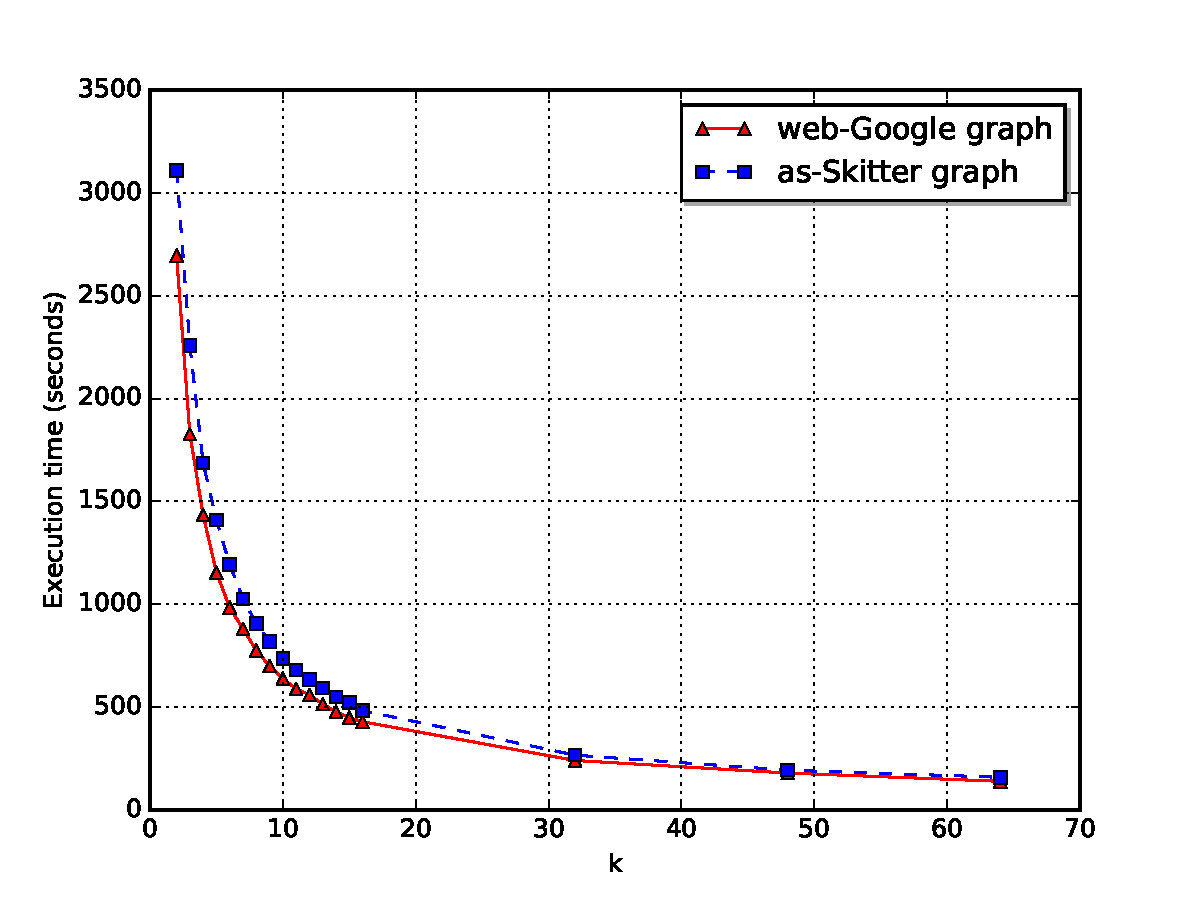
\includegraphics[height=2in,width=2in]{diag}
    \vspace{-0.25in}
    \caption{\scriptsize Performance of the distributed PageRank Algorithm of
	\cite{KlauckNPR15} on two graphs from Stanford Network Analysis Project
	(\url{snap.stanford.edu}): Google Web graph (875713 nodes) and Autonomous
	System by Skitter (1.69M nodes). The algorithm was implemented using MPI and
	run on a cluster of machines interconnected by a high speed network. The
	graph shows that the execution time is proportional (approximately) to
	$\sfrac{1}{k^{0.8}}$.}\label{fig:pr}
\end{figure}

\subsection{Model and Complexity measures}\label{sec:model}
We generalize the \emph{\(k\)-machine} model by incorporating an additional
metric to evaluate the efficiency of algorithms. We first introduce the basic
model (e.g. \cite{KlauckNPR15}) and subsequently introduce our metric.

The standard \(k\)-machine model has \(k\) machines \(M_1, M_2, \hdots, M_k\)
connected together in a clique using bidirectional communication links. The
machines operate in synchronous rounds. The input to this system is a graph
\(G = (V,E)\) with \(|V| = n\) nodes, \(|E| = m\) edges, maximum degree
\(\Delta\), and diameter \(D\). We assume that $n \gg k$, and we focus on the
sublinear regime for $k$, i.e., $k = \bigO{n^{\epsilon}}$, where $0 < \epsilon < 1$
is a constant.\footnote{This is also the assumption in other Big Data parallel
computation models such as the MapReduce and MPC models\cite{soda-mapreduce,MPC}.} 
We assume that each link of the $k$-machine clique has a bandwidth of $B$ bits
per round; we assume $B$ is small compared to the input (graph) size, say,
$B = \Theta(\log n)$ (although one can easily write all bounds in terms of a
general $B$). 

Initially, the entire graph $G$ is not known by any single machine, but rather
partitioned among the $k$ machines in a ``balanced'' fashion, i.e., the nodes
and/or edges of $G$ are partitioned approximately evenly among the machines.
We assume a \emph{vertex-partition} model, whereby vertices, along with
information of their incident edges, are partitioned across machines.
Specifically, the type of partition that we will assume throughout is the
\emph{random vertex partition (RVP)}, that is, each vertex of the input graph is
assigned randomly to one machine.\footnote{There is an alternate partitioning
model, the \emph{random edge partition (REP)} model, where each edge of $G$ is
assigned independently and randomly to one of the $k$ machines. One can relate
the results between the two models~\cite{KlauckNPR15}.} (This is the typical way
used by many real systems, such as Pregel~\cite{pregel}, to initially distribute
the input graph among the machines. See also~\cite{Stanton14,ChingEKLM15}.)


More formally, in the random vertex partition variant, each vertex of $G$ is
assigned independently and uniformly at random to one of the $k$ machines. If a
vertex $v$ is assigned to machine $M_i$, we say that $M_i$ is the \emph{home
machine} of $v$ and, with a slight abuse of notation, write $v \in M_i$. When a
vertex is assigned to a machine, all of its incident edges are assigned to that
machine as well; i.e., the home machine knows the degree of the vertex, the IDs
of the neighbors of that vertex, and the identities of the home machines of the
neighboring vertices (and the weights of the corresponding edges in case $G$ is
weighted). Note that an immediate property of the RVP model is that the number
of vertices at each machine is \emph{balanced}, i.e., each machine is the home
machine of $\softTh{\sfrac{n}{k}}$ vertices with high probability (see \nameref{lem:more-acc-mapping-lemma}).\footnote{Throughout, ``with high
probability", refers to a probability of \(1 - \bigO{1/n}\).} It is assumed that
if a machine knows a vertex ID, it also knows which machine that vertex is
mapped to~\cite{KlauckNPR15}.

Eventually, each machine $M_i$ must set a designated local output variable $o_i$
(which need not depend on the set of vertices assigned to $M_i$), and the
\emph{output configuration} $o=\langle o_1,\dots,o_k\rangle$ must satisfy the
feasibility conditions of the problem at hand. For example, for the minimum
spanning tree problem, each $o_i$ corresponds to a set of edges, and the edges
in the union of such sets must form an MST of the input graph.


Consider an algorithm \(\mathcal{A}\) run on these machines and let \(R_i(\mathcal{A})\), \(1 \leq i \leq k\), denote the total number of communication rounds needed by machine \(M_i\) when running algorithm \(\mathcal{A}\). We define the \emph{communication complexity} of algorithm \(\mathcal{A}\), \(T_c(\mathcal{A})\), as \(T_c(\mathcal{A}) = \max_{i \in [1,k]} R_i(\mathcal{A}).\)

Let \(t_i(\mathcal{A}), 1 \leq i \leq k\) denote the total (sequential) time complexity  for machine \(M_i\) to run \(\mathcal{A}\) across all rounds. Note that the time complexity of a machine
is in the sense of the usual RAM model, i.e., the total time taken by the machine for its (local) computations. We define the \textit{local computation complexity} of algorithm \(\mathcal{A}\), \(T_{\ell}(\mathcal{A})\), by \(T_{\ell}(\mathcal{A}) = \max_{i \in [1,k]} t_i(\mathcal{A})\), i.e., the \emph{worst-case} total local time complexity of a machine.
We would like to minimize $T_{\ell}(\mathcal{A})$ as much as possible; this also is desirable in terms of load balancing (local) computation load among machines (in addition to keeping
the number of communication rounds low). Note that, in general,
if $t(\mathcal{A})$ is  the  running time of algorithm \(\mathcal{A}\)
on \emph{one} machine, i.e., the \emph{sequential} run time, then the best $T_{\ell}(\mathcal{A})$ we can hope for in $k$ machines is $t(\mathcal{A})/k$ (by Amdahl's Law). We note that the overall (wall clock) time needed to solve a problem by an algorithm \(\mathcal{A}\) depends on both \(T_c(\mathcal{A})\)
and \(T_{\ell}(\mathcal{A})\); we specify both individually, since the  time costs for the two measures may differ (typically, a communication ``round'' can take longer than a local computation ``step'').\footnote{We note that in practice, the actual wall clock time might depend on other factors, e.g. the cost of synchronization. In this paper, we focus on  local computation time as an additional important  measure that influences the overall time, besides the traditional communication round complexity measure used to analyze $k$-machine model algorithms.}

Local computation includes the computation time needed by a machine to perform all local operations, including local computation, reading/writing in (local) machine's memory, and communication operations, but {\em excludes}
the time for actual communication between machines (transmitting/receiving messages). For example, if a machine wants to broadcast an $\bigO{\log n}$-sized message to the rest of the machines, then the local computation cost is $\bigO{k}$ (however,
the round complexity for a single broadcast is 1 round and is counted as part of $T_c$). Hence, strictly speaking,
since a machine might send or receive a message to all other machines over the course of the algorithm,
local computation cost is at least $\Omega(k)$. We also assume that the local computation cost
of a machine is at least the cost to read the input assigned to the machine. In the RVP model,
as shown in the \nameref{lem:more-acc-mapping-lemma}.
the number of nodes and edges assigned to a machine is $\Theta(n/k)$ and  $\Omega(m/k+ \Delta)$, respectively,
where $n$ is the number of nodes, $m$ is the number of edges and $\Delta$ is the maximum degree of the input
graph. Thus in our model, the lower bound for $T_{\ell}$ is $\Omega((m+n)/k + \Delta + k)$.

In this paper, we utilize algorithms and theorems related to the synchronous \textsc{Congest} model and the \textsc{Congested Clique} model. The synchronous \textsc{Congest} model is the standard message passing model used to analyze distributed algorithms. Consider a graph \(G=(V,E)\) with \(\card{V}\) nodes and \(\card{E}\) edges. Each node has knowledge of only the edges in \(E\) incident to it but not the complete graph. Each node \(u \in V\) executes a given distributed algorithm in rounds, where each round consists of: (i) receiving messages, if any, sent to it in the previous round; (ii) performing some local computation;
(iii) sending messages, if any, to its neighbors.
Each edge can support messages of size \(\bigO{\log n}\) bits sent across them in a given round.

The \textsc{Congested Clique} model, as defined in~\cite{KlauckNPR15}, acts as an intermediate between the \(k\)-machine model and the standard synchronous \textsc{Congest} model. In addition to the graph \(G=(V,E)\) as defined above, we also consider that nodes in \(V\) are connected in a clique (in a sense, it is the $k$-machine model with $k=n$).
Each node runs a distributed algorithm in rounds as defined above, but can now send and receive messages across all edges in the clique. The bandwidth of each edge is $\bigO{\log n}$ bits of communication per round. As it is, the \textsc{Congested Clique} model is unrealistic for large computations, since $k= n$. 

\subsection{Our Contributions}
We posit a complexity measure called the \emph{local computation cost} (denoted \(T_{\ell}\)) that measures the worst-case local computation
cost among the machines and design and analyze $k$-machine algorithms for two fundamental graph problems, namely connectivity and MST that perform well
under both $T_{\ell}$ and $T_c$ measures. In our model, a natural lower bound on 
\(T_{\ell}\) is $\Omega((m+n)/k + \Delta + k)$ as discussed in \cref{sec:model}.
It is known that a lower bound on the round complexity \(T_c\) is \(\bigOm{n/k^2}\) \cite{KlauckNPR15}. Prior algorithms for connectivity and MST in the $k$-machine model (\cite{KlauckNPR15} and \cite{topc18}; see also the recent algorithm of \cite{gilbert}) do not take into account local computation; straightforward local implementations of them
are not optimal with respect to local computation.  In particular, the algorithm of \cite{topc18} is (essentially) optimal in terms of round complexity (i.e., $\tilde{O}(n/k^2)$),
but its local computation complexity (which was not analyzed in \cite{topc18})  is $\bigO{n^2}$ which is significantly higher than the lower bound of  \(\bigOm{\sfrac{(m+n)}{k}}\).

In this paper, we study several
distributed algorithms for connectivity and MST  and analyze their performance with respect to both the computation
and communication cost for connectivity and MST. The results are summarized in the table on the next page.

We first analyze a well-studied and simple flooding algorithm  for connectivity and connected components that takes \(\softO{n/k+ D}\) rounds and \(\softO{m/k + \Delta}\) local computation time. Flooding algorithms (sometimes called label propagation algorithms) have been studied extensively for finding connected components in a distributed/parallel setting (see e.g., \cite{TianBCTM13} and \cite{aluru}).
However, these algorithms are generally deterministic and are message-intensive. On the
other hand, our algorithm is randomized and is message-efficient. Still, the flooding algorithm
has an inherent bottleneck of taking at least $D$ rounds, where $D$ is the graph diameter.

We next present a natural \emph{deterministic} filtering algorithm for MST (note
that an MST algorithm can be readily used to find connected components by an easy reduction) that has
an improved round complexity of \(\softO{n/k}\) (no dependence on diameter) but has local computation complexity
\(\softO{m/k + n}\), i.e., it is linear in $n$. We then present two \emph{deterministic} MST algorithms which are increasingly sophisticated implementations of the classical Bor\r{u}vka's algorithm, the second of which
has round complexity \(\softO{n/k}\) and local computation complexity \(\softO{(m+n)/k + \Delta + k}\).

We finally present a randomized algorithm to find connected components with
round complexity \(\softO{n/k^2}\) and local computation complexity \(\softO{(m+n)/k + \Delta + k}\) that are both essentially optimal. (Note that in this algorithm, it is only required that each MST edge is output (known) by some machine.)
This algorithm is a better local implementation of the round-optimal algorithm of \cite{PRS21}.
This algorithm is somewhat more involved than the prior algorithms discussed in the paper.
The algorithm, as specified in~\cite{PRS21}, takes at least
$\bigO{n^2}$ local computation time. Our results are summarized in \cref{tbl:results}.
Hence our $k$-machine model algorithms attempt to optimize not only the traditional (communication) round complexity, but also local computation complexity. As mentioned earlier, both determine
the overall performance of an algorithm.


As a byproduct of our analysis, we also present results that
can be useful in analyzing $k$-machine algorithms in general. In particular, we
present a \emph{Node Distribution Lemma} (\cref{lem:node-distribution-lemma})
that is helpful in analyzing local computation complexity in the $k$-machine model.
This lemma can be used to analyze the local computation cost of \textsc{Congest} model
algorithms that are ported in a straightforward way to the $k$-machine model with
a simple  abstraction: if $u$ sends a message to $v$ in the \textsc{Congest} model, then
the machine containing $u$ sends a message to the machine containing $v$ in the
$k$-machine model (see Conversion Theorem in~\cite{KlauckNPR15}).

We also present a \emph{Mapping Lemma} (\cref{lem:more-acc-mapping-lemma})
which gives the distribution of the vertices, edges, and edges per link of the
input graph $G$ with respect to the $k$-clique.

Finally, we mention that the algorithms and analysis presented in the paper will
be useful in efficient implementation in practice. This is left for future work
(discussed in \cref{sec:conclusion}).

\begin{table*}[t]
    \centering
    \begin{tabular}{@{}lll@{}}\toprule
        Algorithm                                                                        & Round complexity            & Local runtime                    \\\midrule
        Flooding  (\cref{sec:congest-connectivity})                               & \(\softO{\frac{n}{k} + D}\) & \(\softO{\frac{m}{k} + \Delta + k}\) \\
        Filtering (\cref{sec:kmachine-filtering-mst})                             & \(\softO{\frac{n}{k}}\)     & \(\softO{\frac{m}{k} + n}\)      \\
        Improved Local Bor\r{u}vka (\cref{sec:boruvka}) & \(\softO{\frac{n}{k}}\)     & \(\softO{\frac{m+n}{k} + \Delta + k}\)        \\
        Randomized Connected Components (\cref{sec:kmachine-mst-optimal})            & \(\softO{\frac{n}{k^2}}\)   & \(\softO{\frac{m+n}{k} + \Delta + k}\)
    \end{tabular}
    \caption{Round Complexity and Local Runtime of Algorithms in the augmented $k$-machine model.}
    \label{tbl:results}
\end{table*}

\section{Preliminaries}

\subsection{Node Distribution Lemma}\label{sec:conv-the}

The Node Distribution Lemma gives a way to bound the parameters associated with
the vertices of an input graph $G$ when it is mapped to the $k$-machine model via
the random vertex partition (RVP) model, where each vertex of the input graph $G$
is assigned independently and uniformly at random among the $k$ machines.
 The parameter of interest can be the degree associated with a vertex or the local computation
cost of a vertex (in the standard \textsc{Congest} model).

\begin{lemma}[Node Distribution Lemma]
    \label{lem:node-distribution-lemma}
    Consider a graph \(G\) of nodes \(v_1, v_2, \hdots, v_n\) with associated non-negative real-valued ``weights'' \(w(v)\) for each node \(v\). Given a uniform, random distribution of the \(n\) nodes to \(k\) machines, as in the \(k\)-machine model, then, with probability at least $1 - \sfrac{1}{n^a}$ for any $a > 0$, the total weight of nodes at every machine is bounded above by $\bigO{T_{\text{avg}}+\log{n}\cdot w_{\max}}$, where \(T_{\text{avg}}=\frac{1}{k}\sum_{i=1}^n w(v_i)\) and \(w_{\max}=\max\set{w(v_i)}\).
\end{lemma}

\begin{proof}
    Partition the nodes into buckets \(\beta_i, 1 \leq i \leq B=\ceil{\log{w_{\max}}} + 1\) based on weight as follows:
	\[\beta_i = \set{v \mid 2^{i-1} \leq w(v) < 2^i}\]
	and set \(\beta_0=\set{v \mid 0 \leq w(v) < 1}\). 
	Furthermore, define \(n_i=\card{\beta_i}\) and let \(B=\ceil{\log{w_{\max}}} + 1\) denote the number of buckets.

	Fix a machine and let \(\mathcal{M}\) denote the set of nodes mapped to it. Furthermore, fix a bucket \(\beta_i=\set{u_1,u_2,\hdots,u_{n_i}}\) and define the random variable \(X_{i,j}\) as
	\[X_{i,j}=\begin{cases}
		1 & \text{ if } u_j \in \mathcal{M}\\
		0 & \text{ otherwise}
	\end{cases}\] Set \(X_i=\sum_{j=1}^{n_i} X_{i,j}\) and note that \(\expectation{X_{i,j}}=\frac{1}{k}\), hence \(\expectation{X_i}=\frac{n_i}{k}\).
	Now, define \[W_i=\sum_{j=1}^{n_i}X_{i,j}w(u_j)\] i.e., \(W_i\) denotes the total weight of nodes in bucket \(\beta_i\) from machine \(M\), and note that \[\prob{W_i > t2^i} \leq \prob{X_i >t}\] Thus, taking \(t = 6\expectation{X_i} + c\log{n}\), we have
	\begin{align*}\prob{W_i > \left(6\expectation{X_i} + c\log{n}\right)2^i}
		&\leq \prob{X_i > 6\expectation{X_i} + c\log{n}}\\
		&\leq 2^{-\left(6\expectation{X_i} + c\log{n}\right)}~\text{\cite{MU17}}\\
		&\leq 2^{-6\expectation{X_i}}\frac{1}{n^c}
	\end{align*}
	Now, notice that
	\begin{align*}\sum_{i=0}^B \left(6\expectation{X_i} + c\log{n}\right)2^i
		&=    \sum_{i=0}^B 6\cdot2^i\frac{n_i}{k} + c\log{n}\sum_{i=0}^B 2^i\\
		&\leq 12\sum_{i=1}^n\frac{w_i}{k} + 4c\log{n}\cdot w_{\max}\\ 
		&=   12T_{\avg} + 4c\log{n}\cdot w_{\max}\\
	\end{align*}
	Taking a union bound across all buckets, we have
	\begin{align*}&\prob{\sum_{i=0}^B W_i > 12T_{\avg} + 4c\log{n}\cdot\ell_{\max}}\\
		&\leq \prob{\sum_{i=0}^B W_i > \sum_{i=0}^B\left(6\expectation{X_i} + c\log{n}\right)2^i}\\
		&\leq \prob{\sum_{i=0}^B X_i > \sum_{i=0}^B 6\expectation{X_i} + c\log{n}}\\ 
		&\leq \sum_{i=0}^B 2^{-6\expectation{X_i}}\frac{1}{n^c}\\
		&\leq \frac{1}{kn^a}\text{ for sufficiently large }c
	\end{align*}
	Taking union bound again across all machines, the probability that any machine has total weight greater than \(12T_{\avg} + 4c\log{n}\cdot w_{\max}\) is bounded above by \(\sum_{i=1}^k\frac{1}{kn^a}=\sfrac{1}{n^a}\). Thus, with probability at least \(1 - \sfrac{1}{n^a}\), every machine has a total weight less than \(12T_{\avg} + 4c\log{n}\cdot w_{\max}\), i.e., all machines have total weight \(\bigO{T_{\avg} + \log{n}\cdot w_{\max}}\) with high probability. 
\end{proof}

\subsection{A More Accurate Mapping Lemma \& Conversion Theorem}\label{sec:more-acc-mapping-lemma}
In this section, we reanalyze the Mapping Lemma from~\cite{KlauckNPR15} (Lemma~4.1 in the reference) in order to develop more exact bounds. The Mapping Lemma gives a bound on the  number 
of vertices and  edges of the input graph $G$ that are mapped to the $k$ machines, assuming
the RVP model. It also gives a bound on the number of edges of $G$ assigned to a link in the $k$-clique. While the first two bounds (the number of vertices and number of edges assigned)
is the same as in \cite{KlauckNPR15}, the bound on the number of edges per link
as stated  and analyzed in \cite{KlauckNPR15} is not fully correct (there the bound was
\(\bigO{m/k^2 + \Delta/k}\), whereas here we show \(\bigO{m/k^2 + n/k}\)).  The analysis in~\cite{KlauckNPR15} also yielded values with hidden polylog terms. We show that a more careful analysis results in no polylog terms. We present the lemma below. 
 The proof uses a powerful (and not well-known) concentration inequality due
to Rodl and Rucinski \cite{RR94} (as used in \cite{PRS21}) which can be of independent interest.

\begin{lemma}[Mapping Lemma]
    \label{lem:more-acc-mapping-lemma}
Let an \(n\)-node, \(m\)-edge graph \(G\) be partitioned among the \(k\) machines as \(N = \set{p_1, \ldots, p_k}\), according to the random vertex partition model (assume \(k = o\left(n\right)\)). Then with probability at least \(1 - 1/n^\alpha\), where \(\alpha > 1\) is an arbitrary fixed constant, the following bounds hold:
\begin{enumerate}
    \item The number of vertices mapped to any machine is \(\bigO{n/k}\).
    \item The number of edges mapped to any machine is \(\mathcal{O}(m/k + \Delta \log n)\).
    \item The number of edges mapped to any link of the network is \(\bigO{m/k^2 + n/k}\).
\end{enumerate}
\end{lemma}

\begin{proof}
    To prove the first bound, recall that nodes are distributed uniformly at random over the machines. Therefore, on expectation, each machine has \(n/k\) nodes. Since $k = \bigO{n^{\epsilon}}$, where $0 < \epsilon < 1$ is a constant, \(n/k = \mathcal{O}(n^{\Omega(1)})\). Thus, we can directly apply a Chernoff bound (the third inequality of Theorem 4.4. from~\cite{MU17}) to see that each machine gets no more than \(6n/k =  \bigO{n/k}\) vertices with the desired probability.

    To prove the second bound, we look back at Lemma~\ref{lem:node-distribution-lemma} and its proof in this paper. If we consider the weights associated with each node to be the local degree of each node, the proof follows directly and we get the desired bound.
    
    To prove the third bound, we utilize the following proposition from~\cite{PRS21}, itself a more accurate version of a proposition from~\cite{RR94}.
    
    \begin{proposition}[Proposition~2 in~\cite{PRS21}]
        \label{prop:edge-bound}
    Let \(G\) be a graph with \(m < \eta n^2\) and let \(R\) be a random subset of \(V\) of size \(\card{R} = t\) such that \(t \geq 1/3\eta\). Let \(e(G[R])\) denote the number of edges in the subgraph induced by \(R\). Then,
        $\prob{e(G[R]) > 3 \eta t^2} < t \cdot e^{-ct}$
    for some \(c > 0\).
    \end{proposition}
    
    Setting \(\alpha = 2\) in our first bound, we see that with probability \(1 - 1/n^2\), each machine gets a random subset of no more than \(6n/k\) nodes. Now, it is easy to see that an upper bound on the number of edges formed by a graph of \(12n / k\) nodes acts as an upper bound on the number of edges mapped to a link between any two machines. We first calculate this upper bound on one link and subsequently extend that bound to all links. We can derive this upper bound by using
    Proposition~\ref{prop:edge-bound} with values \(t =  12n/k\) and \(\eta = m/n^2 + k/n\). Using the proposition, we see that \(\prob{e(G[R]) > O(m/k^2 + n/k)} < 1/n^{\alpha+1}\) for a sufficiently large \(n\).
    
    Now that we have the bound on the number of edges mapped to one link with high probability, we use a simple union bound to see that the number of edges mapped to any link is no more than \(\bigO{m/k^2 + n/k}\) with probability \(1-1/n^\alpha\).
\end{proof}


We are also able to get a more accurate version of the Conversion Theorem from~\cite{KlauckNPR15} (Theorem~4.1 in the reference). As the only changes in the proof are the addition of a \(\log{n}\) factor to account for when \(W=1\) and the direct utilization of the updated bounds from Lemma~\ref{lem:more-acc-mapping-lemma},
 we omit the proof here.

\begin{theorem}[Conversion Theorem]
    \label{thm:more-acc-conversion-theorem}
Suppose that there is an \(\epsilon\)-error algorithm \(A_C\) that solves problem \(P\) in time \(T_C(n) \in \softO{n}\) in the \textsc{Congested Clique} model, for any \(n\)-node input graph. Then there exists an \(\epsilon\)-error algorithm \(A\) that solves \(P\) in the \(k\)-machine model with bandwidth \(W\) satisfying the following time complexity bounds with high probability:
\begin{enumerate}
    \item If \(A_C\) uses point-to-point communication with message complexity \(M\), then \(A\) runs in \(\bigO{(\frac{M}{k^2 W} + T_C(n)\ceil{\frac{n}{kW}}) \log n}\) time.
    \item If \(A_C\) is a broadcast algorithm with broadcast complexity \(B\), then \(A\) takes \(\bigO{\frac{B}{kW} \log n + T_C(n)}\) time.
\end{enumerate}
\end{theorem}

\section{A Parallel Flooding Algorithm for Graph Connectivity}\label{sec:congest-connectivity}
In this section we look at a parallel flooding algorithm to detect whether the input graph is connected and also detect the number of connected components.

We first describe the algorithm from the point of view of individual nodes in a network (as implemented in the standard \textsc{Congest} model) in order to give the intuition behind the process. We subsequently explain how the $k$ machines can simulate this algorithm.

Initially, each node chooses an ID in $[1,n^4]$ uniformly at random. 
For any node $u$, denote the ID of the largest ID $u$ has seen so far as $\textrm{ID-max(u)}$ and initialize this to $u$'s ID. Each node initiates flooding of its ID, in parallel.  Subsequently, if $u$ receives a message containing a higher ID, then $u$ updates its $\textrm{ID-max(u)}$ and floods the new ID.

The above process can be simulated by $k$ machines as follows. Each machine $M$ maintains an ordered list of each node located on the machine, sorted in descending order of ID. $M$ then goes through this list and simulates each node, one by one, as described previously. For a given node $u$ located on $M$, if $u$ has a neighbor $v$ located in machine $M'$, then $M$ sends the appropriate message to $M'$ to be processed.

Let $NR$ refer to the number of rounds it takes for the above process to end
with high probability. Set $NR = \bigO{n\log n/k + D}$.\footnote{In the course
of the proof of \cref{lem:flooding-tc}, we derive this value. Furthermore, a
careful analysis will give us exact values.} After $NR$ rounds, each machine
$M$ aggregates IDs in $\textrm{ID-max(u)}$ for all $u$ located on $M$ into a
list $\mathcal{L}(M)$. The number of IDs in $\mathcal{L}(M)$ indicates the number of distinct components in machine $M$.
Each machine then sends $\mathcal{L}(M)$ to the machine
with the lowest ID in the system, $M_1$. Machine $M_1$ aggregates all such lists
and and counts the number of unique IDs, which is equivalent to the total number
of connected components in the input graph. $M_{\mathrm{lowest}}$ subsequently
broadcasts this number to all other machines.\footnote{While the above algorithm is Monte Carlo in nature, it can be converted into a Las Vegas style algorithm.}
The following theorem captures the properties of this algorithm.

\begin{theorem}
    \label{thm:flooding-thm}
With high probability, the above algorithm correctly counts the number of connected components with \\
$T_{\ell} = \bigO{(m/k + \Delta\log n) \log n + k}$ and $T_c = \bigO{n\log n/k + D}$.
\end{theorem}

\begin{proof}
    We first calculate $T_{\ell}$ and $T_c$ and subsequently argue about the correctness of the algorithm.
    
    In order to calculate $T_c$ and $T_{\ell}$, we first prove the following lemma, which will be used for both calculations.
    
    \begin{lemma}
        \label{lem:num-higher-ids}
    Consider $n$ nodes with IDs chosen uniformly at random from $[1,n^4]$. For any given node $u$, in the \textsc{Congest} model, the number of times it  broadcasts (locally to its neighbors) is $\bigO{\log n}$ with probability at least $1 - 1/n^2$.
    \end{lemma}
    
    \begin{proof}
    For a given node, the probability that at least one other node chooses the same ID as it is $1 - (1- 1/n^4)^n \leq 1/n^3$. By a union bound over all nodes, the probability that at least two nodes have the same ID is $\leq 1/n^2$. Thus, with high probability, all chosen IDs are unique.
    
    Assume, for the sake of analysis,
    that a node $u$ sees each new ID one at a time (since
    if it sees many IDs in one round only the largest ID
    of them will matter). Since
    the IDs are chosen uniformly at random, the IDs can be assumed
    to come in a random permutation order.\footnote{To visualize this, imagine a path of nodes with $u$ at one end where $u$ receives the ID from node at distance $j$ from it in round $j+1$. Let $S$ be the set of IDs chosen by the other nodes. Because each node chooses its ID uniformly at random from $S$, the order in which $u$ receives the other IDs can be seen as a random permutation of the list formed by the elements of $S$.}
    Let $X_i, 1 \leq i \leq n-1$, be the indicator random variable denoting whether the $i^{th}$ ID that $u$ sees (not including its own) causes it to initiate a new local broadcast (this will happen when it sees an ID that
    is higher than the highest one it has seen till now).
    Observe that $\prob{X_i = 1} = 1/i$ and $\prob{X_i = 0} = 1 - 1/i$. Therefore, $\expectation{X_i} = 1/i$. Let $X = \sum_{i=1}^{n-1} X_i$.
    Now $\expectation{\sum_{i=1}^{n-1} X_i} = \sum_{i=1}^{n-1} \expectation{X_i} \leq 4 \log n$. Notice that the $X_i$'s are negatively associated\cite{DubhashiP09}. Thus, we can apply a Chernoff bound\cite{DubhashiP09} and get that $\prob{X > 6\expectation{X}} \leq 1/n^2$.
    
    Thus with probability $1 - 1/n^2$, for a given node $u$, the number of times it broadcasts is $\bigO{\log n}$. 
    \end{proof}
    
    
    We are now ready to calculate $T_{\ell}$ and $T_c$.
    \begin{lemma}
    The local computation complexity of the algorithm is $\bigO{(m/k + \Delta\log n) \log n + k}$ with high probability.
    \end{lemma}
    
    \begin{proof}
    
    We utilize Lemma~\ref{lem:node-distribution-lemma} to bound the local computation complexity. As such, let us first consider running the algorithm on the input graph in the synchronous \textsc{Congest} model. Consider a single node $v_i$ with degree $d(v_i)$. For each value it hears through one of its edges, it must compare that value with the current maximum ID it has seen in $O(1)$ steps of local computation. By Lemma~\ref{lem:num-higher-ids}, each of its $d(v_i)$ neighbors sends it at most $O(\log n)$ values. Thus, $v_i$ performs $\bigO{d(v_i) \log n}$ steps of local computation to process all these messages.
    
    Now, once a value is processed, if the value is higher than $v_i$'s current maximum ID, $v_i$ updates its $\textrm{ID-max}$ and broadcasts this value to its $d(v_i)$ neighbors using $\bigO{d(v_i)}$ steps of local computation. By Lemma~\ref{lem:num-higher-ids}, there are at most $\bigO{\log n}$ values with high probability that $v_i$ will have to broadcast and thus $v_i$ takes an additional $\bigO{d(v_i) \log n}$ steps of local computation to complete these broadcasts.
    
	The maximum run time of any node is thus $\bigO{\Delta \log n}$ with high probability. Therefore, by using Lemma~\ref{lem:node-distribution-lemma} where the weights associated with each node correspond to the maximum run time on that node, with high probability, the local computation of any machine is $\bigO{\frac{1}{k}\left(\sum_{i=1}^n (d(v_i) \log n)\right) + \log n \cdot \Delta \log n} = \bigO{(m / k + \Delta \log n) \log n}$. Finally, there is an additional $k$ due to a machine possibly having to send/read inputs from all other machines resulting in a final local computation complexity of $\bigO{(m / k + \Delta \log n) \log n + k}$.
    \end{proof}
    
    \begin{lemma}
        \label{lem:flooding-tc}
    The communication complexity of the algorithm is $\bigO{n\log n/k + D}$ with high probability.
    \end{lemma}
    
    \begin{proof}
    We bound the total number of broadcasts by $B$. In the \textsc{Congested Clique} model, a broadcast will take $\bigO{D}$ rounds to propagate \emph{over the edges of the input graph}, where $D$ is the diameter of the input graph.
	By \cref{thm:more-acc-conversion-theorem}, we see that the total number of rounds in the $k$-machine model is $\bigO{B\log n/(kW) + D}$ with high probability, where $W$ is the bandwidth of each link in the $k$-machine model. As mentioned in Section~\ref{sec:model}, we assume that the bandwidth of each link is $\Theta(\log n)$, i.e., $W = \Theta(\log n)$.
    
    We show that $B = \bigO{n \log n}$ with high probability. 
    By Lemma~\ref{lem:num-higher-ids}, the number of broadcasts originating at each node is at most $\bigO{\log n}$ with probability $1 - 1/n^2$. 
    Taking a union bound over all nodes, we see that with probability $1 - 1/n$, every node initiates at most $\bigO{\log n}$ broadcasts. Thus, at most $\bigO{n \log n}$ broadcasts are initiated with high probability.
    
    Additionally, every machine $M$ communicates an additional at most $\bigO{n/k}$ labels with high probability, due to transmitting $\mathcal{L}(M)$, to machine $M_{\mathrm{lowest}}$. This is because, initially, each machine receives $\bigO{n/k}$ nodes with high probability, which acts as an upper bound on the number of labels eventually transmitted to $M_{\mathrm{lowest}}$. Thus, we get our desired value of $T_c$.
    \end{proof}
    
    From the construction of the algorithm, it is clear to see that each node $u$ floods any ID it encounters which is higher than the current value of $\textrm{ID-max}$. For each connected component $f$, let $u_f$ be the node with the largest ID in $f$. For each component $f$, after $NR$ rounds, $u_f$ will be flooded to every machine with high probability. It is simple to see that once this has occurred, $M_{\mathrm{lowest}}$ will be able to correctly compute the number of connected components by counting the number of unique IDs from all $\mathcal{L}(M)$ seen.
    \end{proof}

\section{Filtering-based MST Algorithm}\label{sec:kmachine-filtering-mst}
In this subsection, we analyze an algorithm to find a minimum spanning tree (MST) using a filtering technique to eliminate edges   (which was also used  in~\cite{LMSV11}). 

We use three procedures in the course of this algorithm. The first procedure is the well known Kruskal's algorithm  (refer to~\cite{CLRS09}), which when run on a graph with $m$ edges outputs a minimum spanning tree in $\bigO{m\log{m}}$ rounds. 

The second procedure is used to perform matching and is run locally on a machine. It takes a clique of $n$ nodes with unique IDs and outputs a maximal matching in $\bigO{n\log{n}}$ local computation time. First, sort IDs in ascending order using the commonly used MergeSort~\cite{CLRS09}. Then for $i=1$ to $\floor{\sfrac{n}{2}}$, match the $(2i -1)^{th}$ and $(2i)^{th}$ nodes in the sorted list.

The third is the following distributed routing on a clique with $n$ nodes. If each node $u$ wants to send $f$ messages to some other node $\pi(u)$ such that for all $u \neq v, \pi(u) \neq \pi(v)$, then all messages from node $u$ can be sent to $\pi(u)$ in $\bigO{f/(n-1)}$ rounds. The procedure takes two phases. In the first phase, each node $u$ divides its messages into groups of $f/(n-1)$ messages (and appends the destination ID of $\pi(u)$ to each message) and sends these groups of messages across each of its edges, one group per edge, in $\bigO{f/(n-1)}$ rounds. In the second phase, each node forwards whatever messages it received in phase one to the target node in another $\bigO{f/(n-1)}$ rounds.\footnote{The reason we are able to avoid more complicated routing procedures is because (i) each node $u$ sends all its messages to exactly one $\pi(u)$ and (ii) for all $u \neq v, \pi(u) \neq \pi(v)$. As a result, for each edge in the graph, the messages in phase one can be attributed to initial sources and the messages in phase two can be attributed to final destinations. Since each node of an edge can be a source or a destination for exactly one set of $\bigO{f/(n-1)}$ messages, the total number of messages flowing through that edge in either phase is $\bigO{f/(n-1)}$.}

Each machine $M$ maintains graph $G_M$ initially comprising the subgraph induced by edges in $M$, as well as an ordered list $H_M$ initially comprising the IDs of all machines. Each machine $M$ executes at most $2 \ceil{\log k}$ phases of the following steps until termination:
\begin{enumerate}
    \item If $M$ received information about new edges in the previous phase, it updates $G_M$ accordingly. Run Kruskal's algorithm on $G_M$ to remove cycles, if any.
	\item If $|H_M| = 1$, terminate. Use the matching procedure on $H_M$ to match with another machine $M'$. If $M$ matches with $M'$ and the ID of $M$ is greater than the ID of $M'$, use the routing procedure to send $G_M$ to $M'$.
    \item For all machines $M'' \in H_M$ where $M''$ matched with another machine having a lower ID, remove $M''$ from $H_M$. If $M$ was one such $M''$, then terminate.
\end{enumerate}

At the end of algorithm, the machine $M_{min}$ with the lowest ID will have the full MST stored in its $G_{M_{min}}$. The following theorem captures the properties of this algorithm.

\begin{theorem}
    \label{thm:filtering-thm}
	The above algorithm results in the machine with the lowest ID $M_{\min}$ having the full MST stored in its graph $G_{M_{\min}}$ with $T_{\ell} = \bigO{\rho\log{\rho} + n\log{n}\log{k}}$ with high probability, where $\rho = m/k + \Delta \log n$, and $T_c = O(n\log k/k)$.
\end{theorem}

\begin{proof}
We first argue the correctness of the algorithm. In particular, we show that, eventually, information about every edge in the MST of the input graph will be sent to machine $M_{\min}$ before all phases end. Once $M_{\min}$ knows of all these edges, Kruskal's algorithm guarantees that the correct MST will be computed. 

Consider some edge, $e$, of the graph that belongs to the MST. Let $e$ reside on some machine $M$. Because $e$ is an edge of the MST of $G$, $e$ will also be an edge of the MST of any subgraph of $G$ that contains $e$. As a result, $e$ will never be removed by $M$ or any subsequent machine it is located on when Kruskal's algorithm is run. Furthermore, by the matching algorithm, we see that regardless of the initial machine $e$ is located on, after $2 \ceil{\log k}$ phases, it will eventually make its way to machine $M_{\min}$. Thus the algorithm works as intended.

To bound the local computation complexity, observe that any machine $M$ runs for at most $\bigO{\log k}$ phases. 
In any phase, $M$ performs Kruskal's algorithm on graph $G_M$. In the $k$-machine model, by
\cref{lem:more-acc-mapping-lemma}, each machine initially receives $\bigO{m/k + \Delta \log n} = \bigO{\rho}$ edges
with high probability
 resulting in a run time of $\bigO{\rho \log \rho}$ in the first phase. Subsequently, since there are $n$ nodes in the input graph, there can be at most $n-1$ edges chosen by $M$ (or any other machine) to be sent over in that phase. Thus, $M$ processes at most $2n-2$ edges spanning at most $n$ nodes in each subsequent phase resulting in an additional run time of $\bigO{n \log n}$ per phase. Also in each phase, $M$ runs the matching procedure on $H_M$ resulting in at most $\bigO{k \log k}$ steps of local computation. Totally, each machine takes $\bigO{\rho \log \rho + (n \log n  + k \log k)\log k} = \bigO{\rho \log \rho + n \log n \log k}$ steps of local computation with high probability. Note that there is an additive $k$ that comes due to a machine possibly having to send/read inputs from all other machines, but this is subsumed by the larger terms in the complexity.

For the communication complexity, notice as described in the previous paragraph that each machine only needs to send at most $n-1$ edges to another machine it matches with in any give phase. From the matching procedure, this takes $\bigO{n/k}$ rounds per phase. Furthermore, there are at most $\bigO{\log k}$ phases, resulting in a communication complexity of $\bigO{n\log k/k}$.
\end{proof}

\section{Deterministic Bor\r{u}vka-style Algorithms for MST}\label{sec:boruvka}
In this section, we present two \emph{deterministic} distributed algorithms for MST that both have (communication) round complexity of \(\softO{\sfrac{n}{k}}\) and have increasingly better local computation complexity.\footnote{If the graph is connected, the algorithms in this section find an MST. If the graph is disconnected, the algorithms produce a minimum spanning forest (MSF). Note that in an MSF, the number of edges $m$ may be less than the number of nodes $n$.} The  first algorithm (Simple Local Bor\r{u}vka) takes \(\softO{\sfrac{m}{k} +  n}\) local computation time while the second algorithm (Improved Local Bor\r{u}vka) takes \(\softO{\sfrac{m}{k} + \Delta + k}\). 
Note that $\softO{\sfrac{n}{k}}$
is the best possible round complexity if each machine is required to know the MST edges incident on
the vertices assigned to it~\cite{KlauckNPR15}.\footnote{However, if any machine can output any of the MST edges, then the lower bound is $\softOm{n/k^2}$, also shown in \cite{KlauckNPR15}.}
The algorithms are based on a distributed implementation of Bor\r{u}vka's algorithm \cite{Boruvka26,dnabook},  but implemented specifically for the \(k\)-machine model. (Note
that the classical GHS algorithm \cite{GallagerHS83} is a distributed implementation of Bor\r{u}vka in the standard \textsc{Congest} model.) Both algorithms follow a Bor\r{u}vka-style strategy~\cite{Boruvka26}, i.e., repeatedly merge adjacent \emph{components} of the input graph \(G\), which are connected subgraphs of \(G\), to form larger (connected) components (e.g., \cite{dnabook}).

A Bor\r{u}vka-style algorithm proceeds in \emph{phases}. In the first phase, the  algorithm starts with each individual node as a fragment by itself. In subsequent phases, fragments are merged until there is only one remaining --- the MST. That is, at the beginning, there are \(n=\card{V}\) fragments, and at the end of the final phase, a single fragment which is the MST. Throughout, we assume without loss of generality that all edge weights are distinct (if there are duplicate weights, ties can be broken by using the IDs of the endpoints).
At a high level, both algorithms do the following  in each phase:
\begin{enumerate}
    \item For every fragment, its minimum outgoing edge (MOE) is found. An outgoing edge of a fragment is an edge that connects a node of the fragment to a node of a \emph{different} fragment
          and an MOE is an outgoing edge of the least weight. By the cut property, all MOE edges are in the MST. % \cite{}.
    \item Fragments are merged along their MOE edges.
\end{enumerate}
The phases are repeated until all nodes belong to the same fragment.

From the \nameref{lem:more-acc-mapping-lemma}, we note that each machine initially has \(n/k\) nodes distributed randomly (the RVP model), as well as their adjacency lists, and that
the number of edges assigned to each machine is $\bigO{m/k + \Delta \log n}$.  \\

\noindent \textbf{Simple Local Bor\r{u}vka Algorithm.}
Initially, each machine sorts the adjacency list of each node by edge weight, then creates a disjoint-set (or union-find) data structure \cite{CLRS09}, \(\mathcal{M}\), of \emph{fragments}, with \emph{each of the \(n\)} nodes initially belonging to its own fragment. The disjoint-set admits the following operations: (1) \(\operatorname{MakeSet}\) - adds an element to the set in \(\bigO{1}\) time. (2) \(\operatorname{Find}\) - determines which disjoint set an element belongs to in \(\bigO{\invack{n}}\) amortized time (where $\invack{n}$ is the inverse Ackermann function). (3) \(\operatorname{Union}\) - combines disjoint sets in \(\bigO{\invack{n}}\) amortized time.



We note that each machine can easily determine the identities of all \(n\) nodes in \(\bigO{n/k}\) rounds (by executing \(n/k\) broadcasts).

Each phase consists of the following two steps:\\
\textbf{Step 1:} For each vertex \(v\) in machine \(M\), \(M\) iterates through the adjacency list of \(v\) and performs \(\operatorname{Find}\) on each of its neighbors, in increasing order of edge-weight, to determine if the incident edge belongs to a different fragment. Once such an edge is found, \(M\) stops searching and broadcasts this edge to all machines. Note that this search is amortized \(\bigO{\deg{v}}\) local time, as an edge never needs to be checked twice.

Machine $M$ now has a list of candidates for MOE for each fragment. Next, \(M\) notes the minimum candidate for each fragment by iterating through all candidates for each fragment, which it has received from the broadcast mentioned above.\\
\textbf{Step 2:} \(M\) merges fragments: if \((u, v)\) is some minimum outgoing edge between two fragments, \(M\) updates \(\mathcal{M}\) with \(\operatorname{Union}(u, v)\).

At the end of this algorithm, each machine has a local copy of the complete MST.
\begin{theorem}
    \label{thm:gh1}
    The above algorithm ends with \(\mathcal{M}\) as the MST and, with high probability (with respect to the RVP model), we have $T_{\ell} = \softO{\sfrac{m}{k} + n}$ and $T_c = \softO{\sfrac{n}{k}}$.
\end{theorem}


\begin{proof}
    First, note that correctness of this algorithm follows directly from the correctness of Bor\r{u}vka's algorithm.


    Next, note that at the end of each phase, every fragment will merge with at least one other fragment. In the worst case, the number of fragments is halved, hence there are \(\bigO{\log{n}}\) phases, and each phase requires at most \(\bigO{n/k}\) rounds, for a total of $T_c=\bigO{\sfrac{n}{k}\log{n}}=\softO{\sfrac{n}{k}}$.

    Finally, we show the local computation bound. Fix a machine \(M\) and note that pre-processing requires $\bigO{\deg{v}\log{\deg{v}}} = \bigO{\deg{v}\log{\Delta}}$ per node $v$ in \(M\) to sort the adjacency lists. Moreover, to create \(\mathcal{M}\) requires \(\bigO{n}\). In total, this is \(\bigO{\left(\sfrac{m}{k}+\Delta\log{n}\right)\log{\Delta} + n}\) with high probability. The local computation involved in finding the local MOE from Step 1 is amortized \(\bigO{\invack{n}\deg{v}}\) 
    per node, which (by the Mapping Lemma) is \(\bigO{(\sfrac{m}{k} + \Delta \log n) \alpha(n)}\) in total. Finding the MOE per fragment is an additional \(\bigO{n}\) operations. A single instance of Step 2 in a single phase requires \(\bigO{\invack{n}}\) and there can be at most $n-1$ merge operations. Finally, we may have an additive $k$ from a machine possibly having to send/read inputs from all other machines. Thus, we have
	$T_{\ell}=\mathcal{O}(\sfrac{m}{k}\log{\Delta} + \Delta\log{\Delta}\log{n} + n + (m \alpha(n)/k)\linebreak + \Delta \alpha(n) \log n  + n + n \alpha(n)  + k) = \softO{\sfrac{m}{k} + n}$.\qedhere
\end{proof}


\noindent \textbf{Improved Local Bor\r{u}vka Algorithm.}\label{subsec:improved-boruvka}
We can improve the local computation complexity of the Simple Local Bor\r{u}vka algorithm
(which is linear in $n$)  by using a different implementation of Bor\r{u}vka where instead
of broadcast, we simulate the ``unicast" version of Bor\r{u}vka --- as in the GHS algorithm
in the standard \textsc{Congest} model, where  messages are sent through the edges of the graph.
We then use the \nameref{thm:more-acc-conversion-theorem} to compute
the round complexity. However, to get a $\softO{\frac{n}{k}}$ bound (independent of $m$), we first apply filtering to reduce
the number of edges in each machine to $\bigO{n}$ (i.e., $\bigO{nk}$ edges overall) which can be done as follows.

The machines begin by creating a minimum spanning forest (MSF) of their subgraphs using, for example, Kruskal's Algorithm, and essentially discarding edges that are not part of their local MSFs. The edges remaining (of which there are at most \(k\left(n - 1\right)=\bigO{nk}\) with high probability by the Mapping Lemma) are then the only candidates for the MST of the original graph. Moreover, each link between machines corresponds to at most \(\bigO{\sfrac{n}{k}}\) graph edges. The algorithm then continues on these remaining subgraphs.

Like Simple Local Bor\r{u}vka, we proceed in phases. Fix a machine \(M\). To determine the MOE for a fragment \(f\), we first determine the local minimum outgoing edge (LOE) using the following steps. Start with \(\mathrm{LOE}=\infty\), then:\\
\textbf{Step 1:} Iterate through the edges in \(f\). For an edge \((u, v)\) with \(u\) in \(M\), send a message to the machine containing \(v\) with the IDs of \(u\) and \(v\) and the fragment ID of \(f\).\\
\textbf{Step 2:} For each received message \((u, v, f)\), if the fragment ID of \(v\) is different than the received fragment ID, respond with the original fragment ID and the fragment ID of \(v\).\\
\textbf{Step 3:} Update \(\mathrm{LOE} = \min\left(\mathrm{LOE}, w\right)\) for each message received corresponding to fragment \(f\), where \(w\) is the weight of the outgoing edge.\\
\textbf{Step 4:} Broadcast the LOE and fragment ID.

From the broadcast of the LOEs,  each machine locally determines the global MOE for any fragments it contains.

The machine then merges fragments as follows. Note that one cannot merge all fragments,
since that takes time proportional to the length of the fragment chain. To address
this, we use a technique that is similar to (but simpler than) the \emph{controlled GHS} algorithm~\cite{dnabook}.
Create a rooted tree \(F\) where each node is a fragment and there exists an edge between two fragments if there is an MOE between them. Construct a maximal matching (using e.g., Cole-Vishkin~\cite{CV86}) and merge all matched edges \emph{and} any edge where \emph{exactly one} endpoint is matched.

\begin{theorem}
    \label{thm:ghs2}
    With high probability, the above algorithm satisfies $T_{\ell} = \softO{\sfrac{(m + n)}{k} + \Delta + k}$ and $T_c = \softO{\sfrac{n}{k}}$.
\end{theorem}

\begin{proof}
    For local computation, the filtering will require $\mathcal{O}((\sfrac{m}{k}+\Delta)\log{\sfrac{n}{k}})$.
We note that the Cole-Vishkin algorithm (per phase) takes $\bigO{\log^*n}$ rounds
    in the standard \textsc{Congest} model which can be simulated in the $k$-machine model in $\bigO{(n/k)\log^*n}$ rounds since each machine simulates the algorithm for each of
    the $\bigO{n/k}$ vertices assigned to it (apply the broadcast version of
    the \nameref{thm:more-acc-conversion-theorem}). Its local computation cost
    is $\bigO{(n/k)\log^*n}$ since the simulation is done on the MOE edges only, which is $\bigO{n/k}$
    per machine. Additionally, we have an additive $k$ that comes due to a machine possibly having to send/read inputs from all other machines.

    In order to bound the number of total phases, we prove the following lemma.
    \begin{lemma}
        At any step in the given algorithm, the number of sequential merges is at most 3, and the number of total fragments is reduced by at least half after each merge.
    \end{lemma}

    \begin{proof}

        To see that the number of sequential merges is at most 3, simply enumerate all possible labelings of edges (matched or unmatched) on four fragments \(f_1\), \(f_2\), \(f_3\), \(f_4\), with edges from \(f_1\) to \(f_2\), \(f_2\) to \(f_3\), and \(f_3\) to \(f_4\), as well as with one ``outgoing'' edge from each.

        To see that the total number of fragments is reduced by at least half, notice that \emph{every} fragment is part of a merge, for if some fragment \(f\) is not part of a merge, then none of its incident edges are part of the matching \emph{and} none of the edges incident to its neighbors are part of a merge. In that case, we can match an additional edge between the fragment and one of its neighbors, contradicting the maximality of our matching.
    \end{proof}

    By the previous lemma, there are \(\bigO{\log{n}}\) phases in total. Per phase, the overall local computation is clearly $\softO{\sfrac{(m + n)}{k}+\Delta + k}$. In total, this is $\softO{\sfrac{(m+n)}{k}+\Delta + k}$.

    For round complexity, we note that all communication is either via the graph edges
    (as simulated in the $k$-machine model) or by doing $O(n/k)$ broadcasts per phase.
    Round complexity is now obtained by using the Mapping Lemma (where $m = O(nk)$ by filtering) and the Conversion Theorem.
\end{proof}
\section{An Almost-Optimal Randomized  Algorithm}\label{sec:kmachine-mst-optimal}
In this section, we analyze the algorithm for finding connected components presented in~\cite{topc18}.\footnote{An extension  of this algorithm gives an MST algorithm and can be similarly modified as discussed here.} This algorithm is optimal (up to polylogarithmic factors) with respect
to the round complexity (requiring $\softO{n/k^2}$ rounds), but has  $\softO{n^2}$
local computation complexity. However, this algorithm is somewhat more involved than the prior algorithms discussed. For self-containment, we give an overview of the algorithm
of \cite{topc18} and point out why that algorithm has high local computation cost
and discuss the modification needed to obtain the local computation complexity of $\softO{\sfrac{(m+n)}{k} + \Delta + k}$  while keeping the same round complexity. Thus this modified algorithms is essentially optimal (up to polylogarithmic factors)
in both $T_c$ and $T_{\ell}$.

\textbf{Overview.}
The algorithm of \cite{topc18} also follows a Bor\r{u}vka-style strategy~\cite{Boruvka26}, i.e., it repeatedly merges
adjacent \emph{components} of the input graph $G$, which are connected subgraphs of $G$, to form
larger (connected) components. The output of each of these phases is a \emph{labeling} of the nodes of $G$
such that nodes that belong to the same current component have the same label. At the beginning of
the first phase, each node is labeled with its own unique ID, forms a distinct component, and is also the
\emph{component proxy} of its own component. Note that a component proxy is a machine
that is responsible for handling the tasks associated with the component (finding MOE and merging). To load balance communication and computation, the component proxies for each component are chosen randomly among the machines using a 
suitable hash function (see \cite{topc18} for details).  Note that, in any phase, a component contains up
to $n$ nodes, which might be spread across different machines; we use the term \emph{component part}
to refer to all those nodes of the component that are held by the same machine. Hence, in any phase,
every component is partitioned in to at most $k$ component parts. At the end of the algorithm each vertex
has a label such that any two vertices have the same label if and only if they belong to the same connected
component of $G$.

Crucially, the algorithm relies on \emph{linear graph sketches} as a tool to enable communication-efficient
merging of multiple components. Intuitively, a (random) linear sketch $\sketch_u$ of a node $u$'s
graph neighborhood returns a sample chosen uniformly at random from $u$'s incident edges.
Interestingly, such a linear sketch can be represented as matrices using only $\bigO{\polylog(n)}$
bits~\cite{JowhariST11,McGregor14}. A crucial property of these sketches is that they are linear:
that is, given sketches $\sketch_u$ and $\sketch_v$, the \emph{combined sketch} $\sketch_u + \sketch_v$
(``+'' refers to matrix addition) has the property that, with high probability, it yields a random sample of the edges incident to
$(u,v)$ in a graph where we have contracted the edge $(u,v)$ to a single node. 

We now describe how to communicate these graph sketches in an efficient manner\footnote{Linear graph sketches require only $\tilde{O}(1)$ bits of shared randomness which costs
only so much local computation cost and round complexity\cite{topc18}.}:
consider a component $C$ that is split into $j$ parts $P_1,P_2,\dots,P_j$, the nodes of which
are hosted at machines $M_1,M_2,\dots,M_j$. To find an outgoing edge for $C$, we first instruct each
machine $M_i$ to construct a linear sketch of the graph neighborhood of each of the nodes in part $P_i$.
Then, we sum up these $|P_i|$ sketches, yielding a sketch $\sketch_{P_i}$ for the neighborhood of part $P_i$. 
To combine the sketches of the $j$ distinct parts, we now select a \emph{random component proxy}
machine $M_{C,r}$ for the current component $C$ at round $r$.
Next, machine $M_i$ sends $\sketch_{P_i}$ to machine $M_{C,r}$; note that this causes at most $k$ messages
to be sent to the component proxy.\footnote{This requires $\tilde{\Theta}(n/k)$ bits of shared randomness, which can be achieved by having  one machine  generate required bits and subsequently broadcast them. This adds $\Tilde{O}(n/k)$ to the local computation and $\Tilde{O}(n/k^2)$ to the round complexity \cite{topc18}.} Finally, machine $M_{C,r}$ computes $\sketch_C = \sum_{i=1}^j \sketch_{P_i}$,
and then uses $\sketch_C$ to sample an edge incident to some node in $C$, which, by construction, is guaranteed
to have its endpoint in a distinct component $C'$. 

At this point, each component proxy has sampled an inter-component edge
inducing the edges of a \emph{component graph} $\mathcal{C}$ where each vertex corresponds to a component.
To enable the efficient merging of components, the algorithm employs the distributed random ranking technique of~\cite{ChenP12}
to break up any long paths of $\mathcal{C}$ into more manageable directed trees of depth $\bigO{\log n}$.
To this end, each component chooses a rank independently
and uniformly at random from $[0,1]$, and then (virtually) connects to its neighboring
component (according to $\mathcal{C}$) via a (conceptual) directed edge if and only if the latter has a higher rank. 
This process results in a collection of disjoint rooted trees, rooted at the node of highest (local) rank.

The merging of the components of each tree $\mathcal{T}$ proceeds from the leaves upward (in parallel for each tree).
In the first merging phase, each leaf $C_j$ of $\mathcal{T}$ merges with its parent $C'$ by relabeling the component
labels of all of their nodes with the label of $C'$. Note that the proxy $M_{C_j}$ knows the labeling of $C'$,
as it has computed the outgoing edge from a vertex in $C_j$ to a vertex in $C'$.
Therefore, machine $M_{C_j}$ sends the label of $C_j$ to all the machines that hold a part of $C_j$.  This can be done in parallel (for all leaves of all trees) in $\softO{n/k^2}$ rounds.
Repeating this merging procedure $\bigO{\log n}$ times, guarantees that each tree has been merged to a single component. 

Finally, it can be shown that $\bigO{\log n}$ repetitions of the above process suffice to ensure that
the components at the end of the last phase correspond to the connected components of the input graph $G$.

\noindent \textbf{High computation cost of above algorithm.}
The main reason for the high computation cost of the algorithm of \cite{topc18} is the way the algorithm computes
the sketches. It uses the sketches of \cite{JowhariST11,McGregor14} which
defines a vector $\vec{a}_v$ of length $\binom{n}{2}$ for each node $v$ and,
with the appropriate choice of $\mathcal{O}(\log^2{n}) \times \binom{n}{2}$ matrix
$M$, can be used to sample edges. However, doing so requires $\softOm{n^2}$ local
computation time in order to evaluate $M\vec{a}_v$.

\noindent \textbf{Modification to achieve $\softO{\sfrac{(m+n)}{k} + \Delta + k}$ computation complexity.}
The main change needed is, rather than using the sketches of \cite{JowhariST11,McGregor14},
we use the sketch of \cite{KingKT15} (in particular, their \textproc{TestOut} procedure) which also guarantees the same property, i.e., 
finding an MOE with small communication cost. The local computation cost of this procedure
is essentially linear in the size of the component. Rather than storing vectors
of length $\binom{n}{2}$, these sketches utilize an \emph{odd hash function}. In
essence, one of the machines (say the leader machine) determines a
hash function $h:E \to \{0, 1\}$ which is then broadcast to the rest of the
machines.  The hash function is very simple and requires choosing
only two random numbers of $O(1)$ bits\cite{KingKT15}. Next each component
uses this hash function to find an MOE as follows.
Each node in a component part   evaluates $\sum_{\text{incident edges } e} h(e)
\bmod{2}$ and this sum is  first aggregated among the nodes in a component part
by the corresponding machine and then the sums of each part of the component
is aggregated   to the corresponding component proxy machine. 
If the sum is 1, we conclude with some constant probability
$\varepsilon$ that an outgoing edge exists out of the component \cite{KingKT15}. By restricting the edges considered
to be those within some range $[i, j]$, we can (via a routine similar to binary
search) determine a minimum weight outgoing edge with constant probability. By
repeating this process $\bigOm{\log{n}}$ times, we are able to determine the MOE
with high probability for a component and by a union bound (over all components)
determine the MOE of each component with high probability.

By this modification, the local computation cost is linear in the number of edges
assigned to a machine, i.e.,
$\softO{\sfrac{(m+n)}{k} +\Delta + k}$.

\section{Conclusion}
\label{sec:conclusion}
In this paper, we introduced the notion of \textit{local computation} complexity into the $k$-machine model. This notion is important to analyze the performance of large-scale computations in a distributed model, since local computation cost can be a significant factor
in determining the overall (wall-clock) time needed for the algorithm to finish. 

To illustrate the importance of studying such a metric, we analyzed several algorithms in the $k$-machine model and showed that algorithms with similar communication complexities may have vastly different local computation complexities. Thus, we believe that the use of this metric will help the community to better understand the performance of distributed algorithms in practice. 

As part of future work, we plan to implement the algorithms that we analyze in this paper and study their performance in practice. As mentioned in \cref{sec:intro}, we have implemented $k$-machine algorithms for PageRank using the MPI framework.
We plan to do a similar implementation of these algorithms.

It will be interesting to  analyze $k$-machine algorithms (as well as MPC algorithms) using this metric
for other problems.
\bibliography{references}
\bibliographystyle{plain}
\end{document}